\subsection{Kiểm chứng điểm đau (Pain Point Validation):}
\subsection{Đề xuất giải pháp sơ bộ (Proposed Solution):}
\subsubsection{Ý tưởng giải pháp}
\subsubsection{Quy trình đề xuất (To-Be Process)}
\subsubsection{Tính khả thi}
\begin{table}[H]
    \centering % Lệnh này sẽ tự động căn giữa bảng 0.9\textwidth
    \renewcommand{\arraystretch}{1.6}
    % Định nghĩa cột C căn giữa, cột X căn lề đều
    \newcolumntype{C}{>{\centering\arraybackslash}m{2.5cm}}
    \newcolumntype{D}{>{\centering\arraybackslash}m{2cm}}
    
    \begin{tabularx}{0.9\textwidth}{|C|D|X|} % Thu hẹp độ rộng bảng còn 90%
        \hline
        \rowcolor[HTML]{EFEFEF} 
        \textbf{KHÍA CẠNH} & \textbf{ĐÁNH GIÁ} & \centering\arraybackslash \textbf{CHI TIẾT} \\ \hline
        
        \textbf{Kỹ thuật} & Khả thi & Sử dụng các công nghệ phổ biến như \textbf{LLM (OpenAI/Gemini)}, \textbf{FastAPI} và \textbf{Firebase}. Các chức năng chính như sửa lỗi ngữ pháp, sinh bài tập, lưu tiến độ đều đã có API hỗ trợ. \\ \hline
        
        \textbf{Kinh tế} & Khả thi & Chi phí thấp do có thể dùng API miễn phí hoặc \textbf{free tier} (Gemini, Firebase). Chi phí chủ yếu là thời gian phát triển. \textbf{ROI cao} về mặt học tập và demo dự án. \\ \hline
        
        \textbf{Thời gian} & Khả thi & Có thể hoàn thành trong \textbf{8-9 tuần} nếu chia nhỏ chức năng: (1) core AI sửa lỗi, (2) sinh bài tập, (3) giao diện game đơn giản. \\ \hline
        
        \textbf{Vận hành} & Khả thi & Hệ thống đơn giản, dễ triển khai (\textbf{web/mobile}). Backend nhẹ, không cần xử lý real-time phức tạp. Có thể deploy bằng các nền tảng miễn phí. \\ \hline
    \end{tabularx}
    \caption{Bảng đánh giá tính khả thi của đồ án}
    \label{tab:tinh-kha-thi}
\end{table}
\subsubsection{Các tính năng chính (Core Features)}
\begin{itemize}[label=-]
\item \textbf{Interactive AI NPCs (Giao tiếp với nhân vật ảo):} 
Người chơi trò chuyện trực tiếp với các NPC được tích hợp LLM để nhận nhiệm vụ và thực hành tiếng Anh, giải quyết tình trạng thiếu môi trường giao tiếp thực tế.

\item \textbf{Real-time Grammar Correction:} 
Hệ thống tự động phát hiện và hướng dẫn sửa lỗi ngữ pháp ngay trong lúc người chơi đang "chat" với NPC, giải quyết vấn đề người học không biết mình sai ở đâu khi giao tiếp.

\item \textbf{Dynamic Vocabulary Notebook:} 
Ghi nhận từ vựng mới vào túi đồ (Inventory/Notebook) và AI sẽ chủ động lồng ghép lại các từ này vào lời thoại của NPC trong các bối cảnh sau, giải quyết việc học từ rời rạc, dễ quên.

\item \textbf{Adaptive Quest System (Hệ thống nhiệm vụ thích ứng):}
Tự động sinh ra các thử thách, bài tập (điền từ, giải đố) dưới dạng "Nhiệm vụ trong game" (Quests) dựa trên lỗi sai lịch sử của người chơi, giải quyết việc luyện tập không cá nhân hóa.

\item \textbf{Error Tracking \& Boss Review:} 
Lưu lại "bệnh án" lỗi sai và tái sử dụng chúng làm chướng ngại vật hoặc câu hỏi khi đánh Boss định kỳ, giải quyết việc lặp lại lỗi cũ mà không có động lực cải thiện.
\end{itemize}
Dưới đây là sơ đồ minh họa chi tiết kiến trúc hệ thống 3 lớp (3-tier architecture) của đồ án, thể hiện rõ luồng tương tác giữa người chơi (Frontend), các module xử lý AI tại Backend (FastAPI) và hệ thống lưu trữ dữ liệu (Firebase).
\begin{figure}[H]
    \centering
    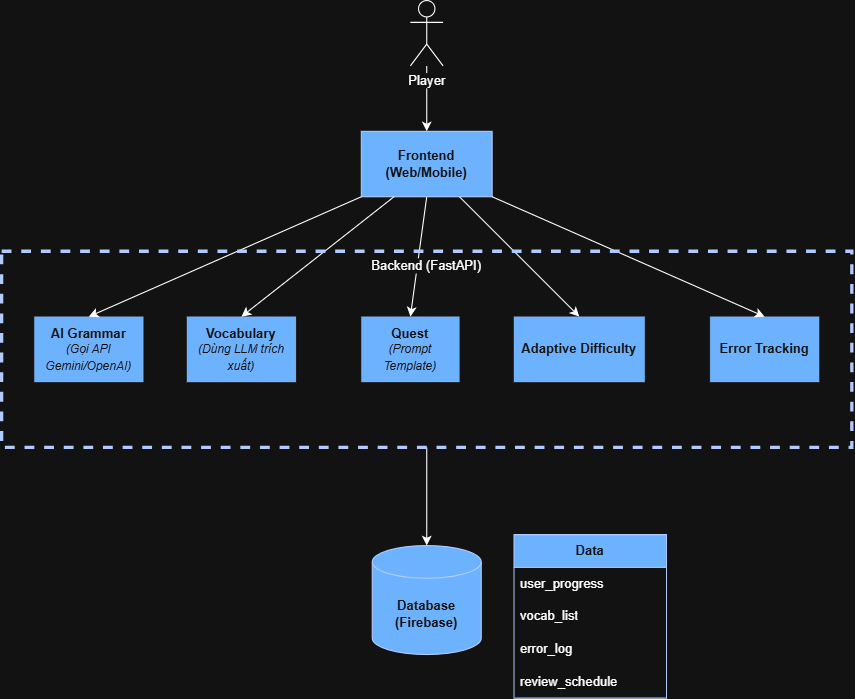
\includegraphics[width=0.9\textwidth]{Figure/architecture_map.png}
    \caption{Minh họa thêm kiến trúc hệ thống}
    \label{fig:arch-map}
\end{figure}
\subsection{Rủi ro (Risks)}
\renewcommand{\arraystretch}{1.6} 
\newcolumntype{S}{>{\centering\arraybackslash}m{0.8cm}} 
\newcolumntype{C}{>{\centering\arraybackslash}m{2cm}}   
\newcolumntype{P}{>{\raggedright\arraybackslash}X}      

\begin{xltabular}{\textwidth}{|S|P|P|C|C|P|}
    % Caption và Label phải đặt ở ĐẦU bảng trong xltabular
    \caption{Bảng phân tích rủi ro dự án (Risk Matrix)}
    \label{tab:rui-ro} \\
    \hline
    
    % --- ĐÂY LÀ PHẦN TIÊU ĐỀ CHO TRANG ĐẦU TIÊN ---
    \rowcolor[HTML]{EFEFEF} 
    \textbf{STT} & \centering\arraybackslash \textbf{RỦI RO} & \centering\arraybackslash \textbf{NGUYÊN NHÂN} & \textbf{KHẢ NĂNG XẢY RA (1-5)} & \textbf{TÁC ĐỘNG (1-5)} & \centering\arraybackslash \textbf{BIỆN PHÁP PHÒNG NGỪA} \\ \hline
    \endfirsthead
    
    % --- ĐÂY LÀ PHẦN TIÊU ĐỀ SẼ TỰ ĐỘNG LẶP LẠI NẾU BẢNG BỊ CẮT SANG TRANG 2 ---
    \hline
    \rowcolor[HTML]{EFEFEF} 
    \textbf{STT} & \centering\arraybackslash \textbf{RỦI RO} & \centering\arraybackslash \textbf{NGUYÊN NHÂN} & \textbf{KHẢ NĂNG XẢY RA (1-5)} & \textbf{TÁC ĐỘNG (1-5)} & \centering\arraybackslash \textbf{BIỆN PHÁP PHÒNG NGỪA} \\ \hline
    \endhead
    
    % --- NỘI DUNG BẢNG ---
    1 & Người dùng không muốn sử dụng lâu dài & Game chưa đủ hấp dẫn, thiếu động lực & 4 & 4 & Thêm game hóa (quest, level, reward), thiết kế UI đơn giản, có daily quest \\ \hline
    
    2 & AI sửa lỗi không chính xác & Prompt chưa tốt, model hạn chế & 3 & 5 & Tối ưu prompt, kiểm tra output, giới hạn dạng bài (chỉ grammar cơ bản) \\ \hline
    
    3 & Hệ thống hoạt động chậm & Gọi API AI có độ trễ & 3 & 3 & Xử lý async, loading UI, tối ưu request \\ \hline
    
    4 & Thiếu dữ liệu để cá nhân hóa & Ít người dùng hoặc ít tương tác & 2 & 3 & Dùng rule-based ban đầu, lưu toàn bộ lịch sử người dùng \\ \hline
    
    5 & Người dùng nhập sai quá nhiều (input lỗi) & Trình độ thấp hoặc nhập linh tinh & 3 & 3 & Giới hạn input, gợi ý câu mẫu, validate dữ liệu đầu vào \\ \hline
    
    6 & Scope quá lớn, không kịp deadline & Thêm quá nhiều tính năng & 4 & 5 & Giới hạn chỉ vocab + grammar, ưu tiên core features trước \\ \hline
    
\end{xltabular}
\textbf{Công thức tính mức độ ưu tiên rủi ro:}
Dựa vào điểm số (Score), mức độ ưu tiên xử lý rủi ro được phân loại như sau:
\begin{itemize}[label=$\bullet$]
    \item \textbf{Score $\geq$ 12:} Ưu tiên cao (Cần có biện pháp xử lý và theo dõi sát sao).
    \item \textbf{Score từ 8 - 11:} Ưu tiên trung bình (Cần chuẩn bị sẵn phương án dự phòng).
    \item \textbf{Score $<$ 8:} Ưu tiên thấp (Chấp nhận rủi ro và theo dõi định kỳ).
\end{itemize}
\subsection{Tiêu chí thành công (Success Criteria)}
\subsubsection{Chỉ số định lượng (Quantitative Metrics)}
\begin{itemize}[label=-]
\item \textbf{Hiệu suất:} Thời gian phản hồi AI (sửa lỗi + sinh bài tập) $\leq$ 5 giây.
\item \textbf{Sử dụng:} $\leq$ 70$\%$ người dùng quay lại ít nhất 2 lần/tuần.
\item \textbf{Hiệu quả học tập:} Điểm bài test ngữ pháp/từ vựng tăng $\geq$ 25$\%$ sau 2 tuần sử dụng.
Hoàn thành nhiệm vụ: $\geq$ 80$\%$ quest được hoàn thành mỗi phiên chơi.
\item \textbf{Độ chính xác AI:} $\geq$ 90$\%$ câu sửa ngữ pháp được đánh giá đúng.
\item \textbf{Lỗi hệ thống:} Tỷ lệ lỗi (API fail, crash) $<$ 3$\%$.
\end{itemize}
\subsubsection{Chỉ số định tính (Qualitative Metrics)}
\begin{itemize}[label=-]
\item Người dùng cảm thấy việc học tiếng Anh \textbf{thú vị hơn so với cách truyền thống}.
\item Người học \textbf{hiểu rõ lỗi sai của mình} thay vì chỉ biết đúng/sai.
\item Trải nghiệm game giúp \textbf{tăng động lực học lâu dài}.
\item Người dùng đánh giá hệ thống \textbf{dễ sử dụng, thân thiện}.
\item Nội dung học được cảm nhận là \textbf{cá nhân hóa (đúng điểm yếu của mình)}.
\end{itemize}
\subsubsection{Cách đo lường}
\begin{itemize}[label=-]
\item \textbf{Khảo sát trước, sau khi sử dụng:} đo mức cải thiện kiến thức và mức độ hài lòng.
\item \textbf{System Logs (Firebase):} theo dõi số lần đăng nhập, thời gian sử dụng, tần suất làm quest.
\item \textbf{AI evaluation:} so sánh output AI với tập câu chuẩn để đo độ chính xác.
\item \textbf{Tracking tiến độ học:} lưu lịch sử đúng/sai để đo improvement ($\%$).
\item \textbf{Phỏng vấn người dùng:} thu thập feedback về trải nghiệm và mức độ hứng thú.
\end{itemize}